\documentclass[a4 paper]{article}
% Set target color model to RGB
\usepackage[inner=2.0cm,outer=2.0cm,top=2.5cm,bottom=2.5cm]{geometry}
\usepackage{setspace}
\usepackage[rgb]{xcolor}
\usepackage{verbatim}
\usepackage{subcaption}
\usepackage{amsgen,amsmath,amstext,amsbsy,amsopn,tikz,amssymb,tkz-linknodes}
\usepackage{fancyhdr}
\usepackage[colorlinks=true, urlcolor=blue,  linkcolor=blue, citecolor=blue]{hyperref}
\usepackage[colorinlistoftodos]{todonotes}
\usepackage{rotating}
%\usetikzlibrary{through,backgrounds}
\hypersetup{%
pdfauthor={Ashudeep Singh},%
pdftitle={Assignment 4},%
pdfkeywords={Tikz,latex,bootstrap,uncertaintes},%
pdfcreator={PDFLaTeX},%
pdfproducer={PDFLaTeX},%
}
%\usetikzlibrary{shadows}
% \usepackage[francais]{babel}
\usepackage{booktabs}
\newcommand{\ra}[1]{\renewcommand{\arraystretch}{#1}}

\newtheorem{thm}{Theorem}[section]
\newtheorem{prop}[thm]{Proposition}
\newtheorem{lem}[thm]{Lemma}
\newtheorem{cor}[thm]{Corollary}
\newtheorem{defn}[thm]{Definition}
\newtheorem{rem}[thm]{Remark}
\numberwithin{equation}{section}

\newcommand{\homework}[6]{
   \pagestyle{myheadings}
   \thispagestyle{plain}
   \newpage
   \setcounter{page}{1}
   \noindent
   \begin{center}
   \framebox{
      \vbox{\vspace{2mm}
    \hbox to 6.28in { {\bf COMP 3005:~Database Management Systems \hfill {\small (#2)}} }
       \vspace{6mm}
       \hbox to 6.28in { {\Large \hfill #1  \hfill} }
       \vspace{6mm}
       \hbox to 6.28in { {\it Instructor: {\rm #3} \hfill Name: {\rm #5}, ID: {\rm #6}} }
       %\hbox to 6.28in { {\it TA: #4  \hfill #6}}
      \vspace{2mm}}
   }
   \end{center}
   \markboth{#5 -- #1}{#5 -- #1}
   \vspace*{4mm}
}

\newcommand{\problem}[2]{~\\\fbox{\textbf{Q #1}}\hfill (#2 points)\newline\newline}
\newcommand{\subproblem}[1]{~\newline\textbf{(#1)}}
\newcommand{\D}{\mathcal{D}}
\newcommand{\Hy}{\mathcal{H}}
\newcommand{\VS}{\textrm{VS}}
\newcommand{\solution}{~\newline\textbf{\textit{(Solution)}} }

\newcommand{\bbF}{\mathbb{F}}
\newcommand{\bbX}{\mathbb{X}}
\newcommand{\bI}{\mathbf{I}}
\newcommand{\bX}{\mathbf{X}}
\newcommand{\bY}{\mathbf{Y}}
\newcommand{\bepsilon}{\boldsymbol{\epsilon}}
\newcommand{\balpha}{\boldsymbol{\alpha}}
\newcommand{\bbeta}{\boldsymbol{\beta}}
\newcommand{\0}{\mathbf{0}}



\begin{document}
\homework{Assignment \#5}{Due: Friday Dec. 10, 2021 (11:59 PM)}{Ahmed El-Roby}{}{Ryan Lo}{101117765}
\textbf{Instructions}: Read all the instructions below carefully before you start working on the assignment, and before you make a submission.
\begin{itemize}
    \item The accepted format for your submission is pdf. 
    \item If you use the tex file, make sure you edit line 28 to add your name and ID. Only write your solution and do not change anything else in the tex file. If you do, you will be penalized.
    %\item All questions in this assignment use the university schema discussed in class (on culearn), unless otherwise stated.
    %\item For SQL questions, upload a text file with your queries in the format shown in the file ``template.txt'' uploaded on culearn. An example submission is in the file ``sample.txt''. You will be penalized if the format is incorrect or there is no text file submission.
    %\item For programming questions, upload your .java file.
    \item Late submissions are allowed for 24 hours after the deadline above with a penalty of 10\% of the total grade of the assignment. Submissions after more than 24 are not allowed.
\end{itemize}

\problem{1:}{4}
RAID systems can support replacing failed disks without the system going offline. Which of the RAID levels better support this operation with the least amount of interference between the rebuild and ongoing disk accesses? Explain your answer.

RAID level 1 (reflecting) is the one which facilitates rebuilding of a failed disk with least interference with the on-going disk accesses. 
In the case where a drive fails, the data does not have to rebuild itself, since In RAID level 1 you have two copies of the data itself,
the data just has to be copied to the replacement drive.

\problem{2:}{4}
Consider the following arrangement for four disks, where $B_{i}$ is a data block, and $P_{i}$ is the parity block for the 4 data blocks that precedes it. What problem will this arrangement cause?

{\centering 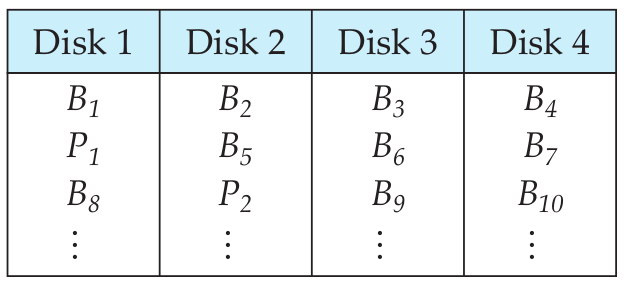
\includegraphics[width=\textwidth/2]{figure1.png}}

This arrangement of parity blocks is more prune to losing information if some blocks get corrupted.
Since some of the rows in the disk arrangement does not include a parity block, blocks in those rows 
would be hard to recover if those blocks were to be corrupted.

\problem{3:}{8}
Consider the following file organization using free list.

{\centering 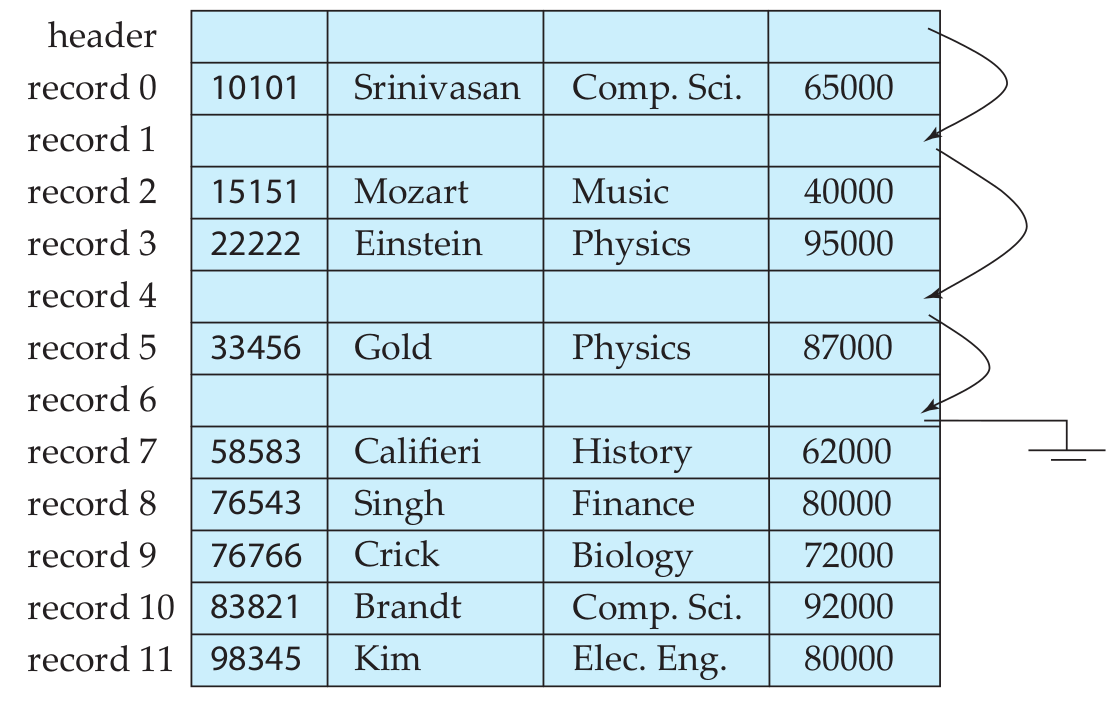
\includegraphics[width=\textwidth/2]{figure2.png}}

Show the structure of the file after each of the following operations (\textbf{they follow one another}):

\subproblem{a} Delete record 11.\indent (2 marks)

{\centering \includegraphics[width=\textwidth/2]{figure2 - copy.png}}

\subproblem{b} Insert (12345, John, History, 90000) (3 marks)

{\centering 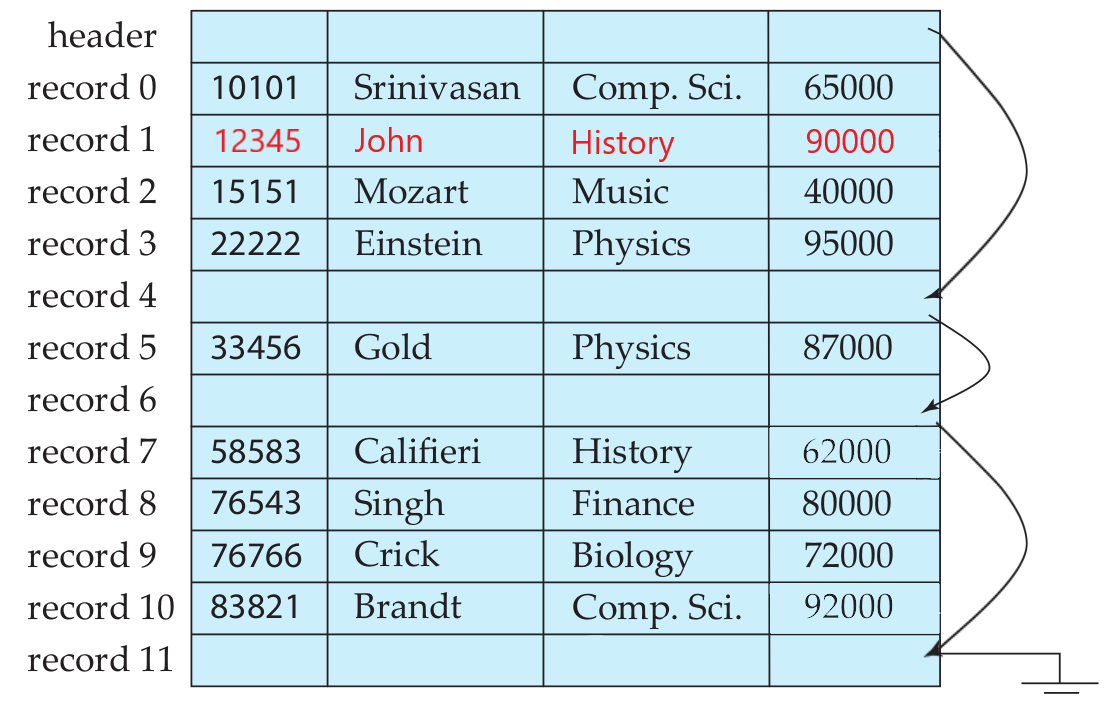
\includegraphics[width=\textwidth/2]{figure2 - Copy - Copy.png}}

\subproblem{c} Insert (20000, Jamie, Physics, 100000).\indent (3 marks)

{\centering 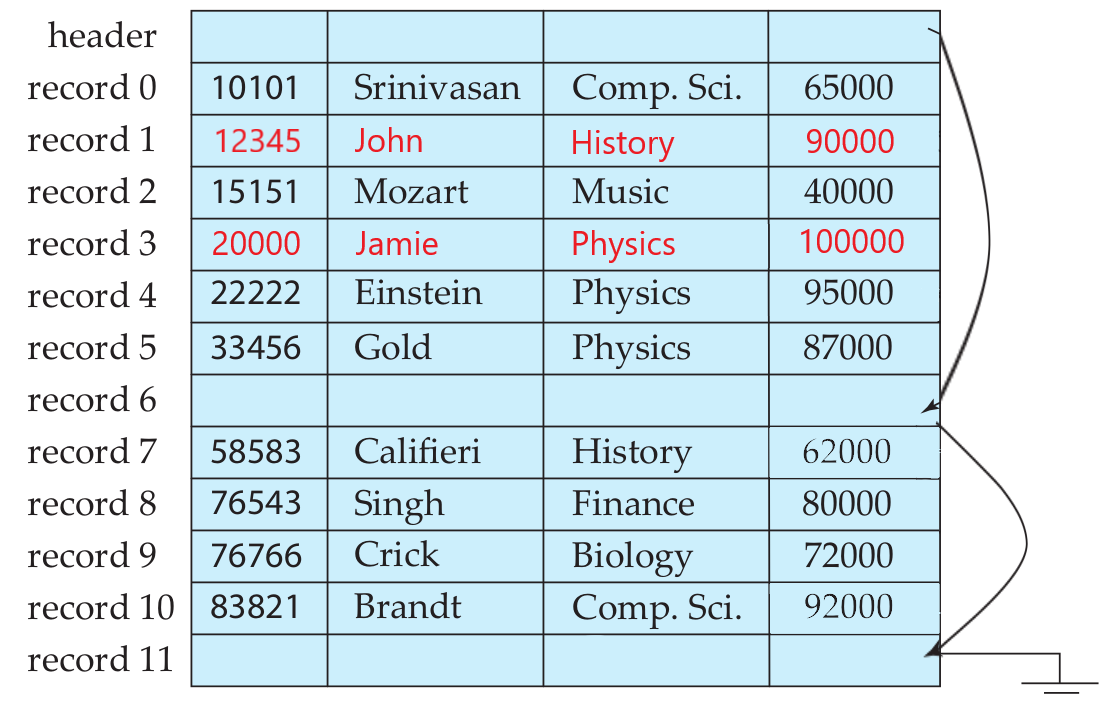
\includegraphics[width=\textwidth/2]{figure2 - Copy - Copy - Copy.png}}

\problem{4:}{3}
In variable-length record representation, the record starts with offset and length pairs of variable-size attributes, followed by fixed-size attributes, then the null bitmap, and finally the variable-size attributes. How can we improve this representation if our application is expected to store tables with large number of attributes, most of which are nulls?

This representation could be improved if expected to store tables with large number of attributes and most of which are nulls by
keeping the null bitmaps updated.

\problem{5:}{12}
Construct a $B^{+}$-tree for the following set of key values: (2, 3, 5, 7, 11, 17, 19, 23, 29, 31). The tree is initially empty and values are added one value at a time in ascending order. Consider the following values of $n$:
\subproblem{a} $n = 4$.\indent \indent (4 points)

{\centering 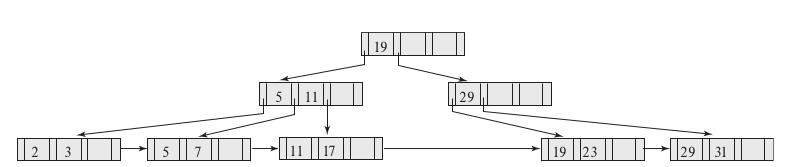
\includegraphics[width=\textwidth/2]{tree-delete - Copy.png}}

\subproblem{b} $n = 6$.\indent \indent (4 points)

{\centering 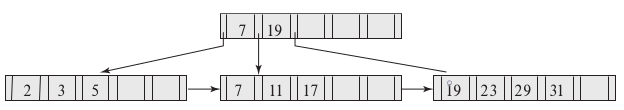
\includegraphics[width=\textwidth/2]{tree-insert - Copy.png}}

\subproblem{c} $n = 8$.\indent \indent (4 points)

{\centering 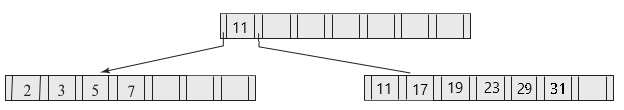
\includegraphics[width=\textwidth/2]{tree-insert - Copy - Copy.png}}

\newpage

\problem{6:}{8}
Consider the following $B^{+}$-tree with $n = 4$:
\begin{figure}[h]
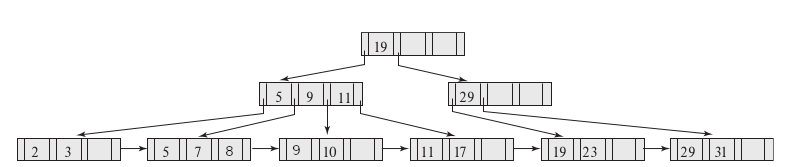
\includegraphics[height=2in, width=6in]{tree-delete.png}
\end{figure}

\subproblem{a} Delete 23.\indent \indent (4 points)

{\centering 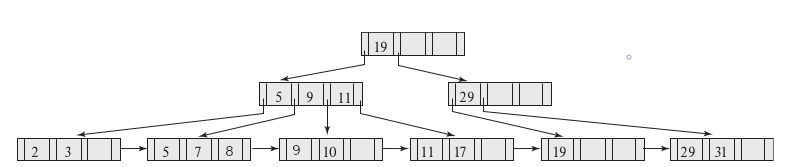
\includegraphics[width=\textwidth/2]{tree-delete - Copy (2).png}}

\subproblem{b} Delete 19 (after the previous deletion in (a)).\indent \indent (4 points)

{\centering 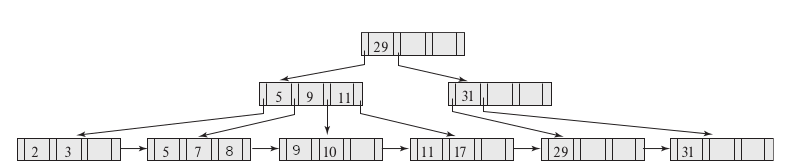
\includegraphics[width=\textwidth/2]{tree-delete - Copy (2) - Copy.png}}

\problem{7:}{4}
Consider the following $B^{+}$-tree with $n = 6$:
\begin{figure}[h]
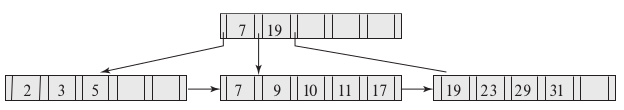
\includegraphics[height=1in, width=5in]{tree-insert.png}
\end{figure}
Insert 8 into this tree.

{\centering 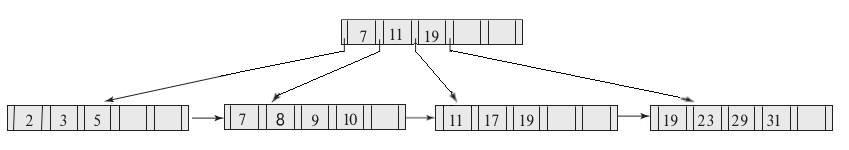
\includegraphics[width=\textwidth/2]{tree-insert - Copy (2).png}}


\end{document}

